{\let\clearpage\relax
\chapter{Mô hình hóa bài toán quy hoạch mở rộng nguồn điện}}
\label{chap:problem-modeling}

Dựa trên các nền tảng lý thuyết đã được trình bày ở Chương 2, chương này đi sâu vào việc xây dựng và công thức hóa bài toán cốt lõi của đề tài: Bài toán GEP giải quyết bằng kiến trúc tối ưu hóa lai hai cấp. Cách tiếp cận này giúp xử lý không gian tìm kiếm rộng lớn và tính bất định của năng lượng tái tạo, đồng thời duy trì các ràng buộc vận hành tuyến tính trong phạm vi mô hình được xây dựng.

% ================================================================
\section{Khung mô hình tối ưu hóa lai hai cấp}
% ================================================================

Bài toán quy hoạch mở rộng nguồn điện vốn yêu cầu xem xét đồng thời quyết định đầu tư dài hạn (xây nhà máy gì, ở đâu, công suất bao nhiêu) và quyết định vận hành ngắn hạn (huy động các nhà máy như thế nào để đáp ứng phụ tải từng giờ). Để giải quyết bài toán này một cách khả thi và hiệu quả, đề tài đề xuất phân tách bài toán thành cấu trúc hai cấp:

\begin{itemize}
    \item \textbf{Cấp trên:} Đóng vai trò hoạch định chiến lược đầu tư. Cấp này sử dụng các thuật toán Trí tuệ nhân tạo (Học tăng cường hoặc Tối ưu hóa Bayes) để tìm kiếm và đề xuất các phương án đầu tư công suất (véctơ $\mathbf{x}$).
    \item \textbf{Cấp dưới:} Đóng vai trò mô phỏng điều độ hệ thống. Cấp này nhận phương án đầu tư từ cấp trên, cập nhật cấu trúc lưới điện, và giải bài toán LP để mô phỏng vận hành hệ thống trong suốt một năm (hoặc các ngày đại diện). Cấp dưới sau đó sẽ trả về kết quả là chi phí vận hành và lượng cắt tải (nếu có) cho cấp trên.
\end{itemize}

Vòng lặp tương tác giữa hai cấp giúp các thuật toán ở cấp trên dần dần nhận diện những phương án đầu tư có điểm phạt thấp, dựa trên phản hồi chi phí vận hành và cắt tải từ bài toán LP cấp dưới.

\textbf{Giả thiết tuyến tính hóa:} Để đảm bảo tính khả thi tính toán, đề tài tuyến tính hóa bài toán vận hành ở cấp dưới dưới dạng LP. Cụ thể, cân bằng công suất, giới hạn phát, giới hạn truyền tải liên vùng và biến cắt tải đều được mô tả bằng các ràng buộc tuyến tính. Cấp trên không được xem như một LP tường minh, vì chi phí vận hành và lượng cắt tải chỉ xuất hiện sau khi giải bài toán vận hành ở cấp dưới. Do đó, cấp trên được xử lý như một bài toán tối ưu không đạo hàm trên hàm mục tiêu hộp đen sinh ra từ lời giải cấp dưới. Cách tiếp cận này chấp nhận giảm bớt độ chi tiết so với mô hình phi tuyến đầy đủ nhưng đổi lại cho phép đánh giá lặp lại nhiều phương án đầu tư trên hệ thống quy mô lớn. Phương pháp KKT-LP tương ứng là một quy tắc quy hoạch cận biên dựa trên trực giác đối ngẫu của bài toán vận hành tuyến tính, được trình bày chi tiết trong các phần sau.

\begin{figure}[!ht]
    \centering
    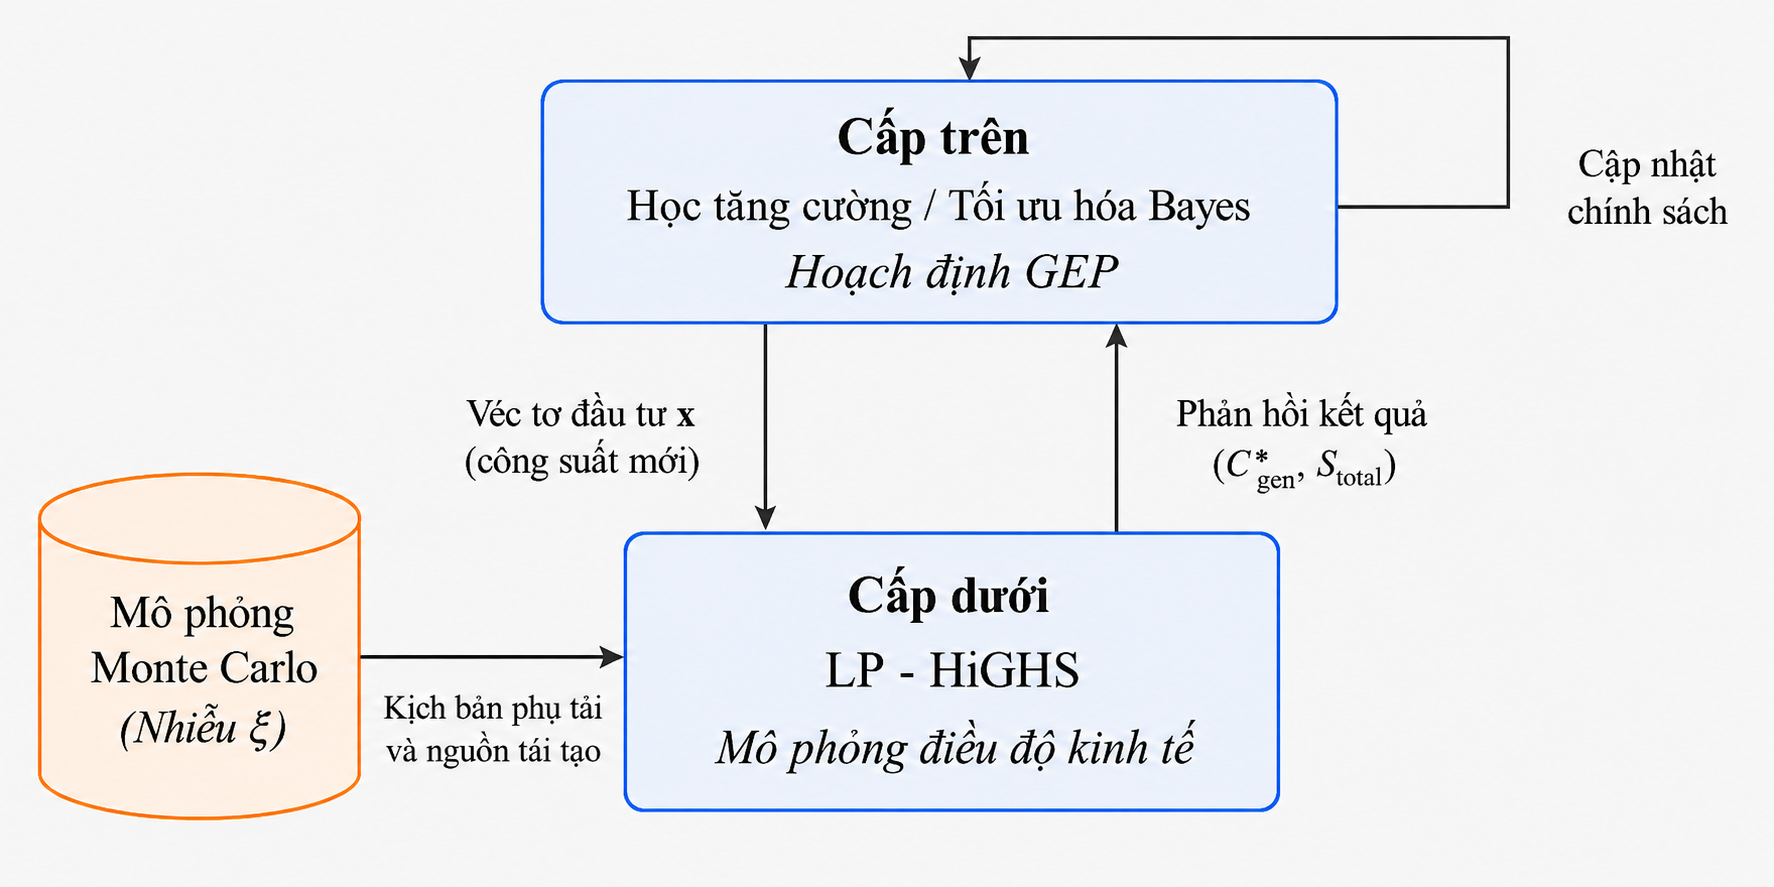
\includegraphics[width=\textwidth]{images/pipeline.png}
    \caption{Sơ đồ luồng thông tin trong kiến trúc tối ưu hóa lai hai cấp}
    \label{fig:bilevel_flow}
\end{figure}
% ================================================================
\section{Mô hình toán học cấp dưới cho bài toán điều độ kinh tế}
% ================================================================

Mục tiêu của bài toán cấp dưới là tối thiểu hóa chi phí điều độ trong từng giờ, trong đó biến cắt tải được gắn hệ số VOLL để mô hình vẫn có nghiệm khả thi khi cung không đủ cầu. Khi tổng hợp ở cấp trên, lượng cắt tải được lưu riêng như một chỉ tiêu độ tin cậy.

\subsection{Tập hợp, tham số và biến quyết định}

\textbf{Tập hợp:}
\begin{itemize}
    \item $\mathbf{Z}$: Tập hợp các vùng trong hệ thống, chỉ số $z$.
    \item $\mathbf{G}$: Tập hợp tất cả các máy phát điện (bao gồm cả hiện hữu và xây mới), chỉ số $i$. $\mathbf{G}_z$ là tập các máy phát thuộc vùng $z$.
    \item $\mathbf{L}$: Tập hợp các đường dây truyền tải liên kết giữa các vùng, chỉ số cặp $(z, z')$.
    \item $\mathbf{T}$: Tập hợp các khung giờ vận hành trong năm mô phỏng, chỉ số $t$.
\end{itemize}

\textbf{Tham số:}
\begin{itemize}
    \item $D_z^t$: Nhu cầu phụ tải tại vùng $z$ trong giờ $t$ (MW).
    \item $P_i^{\max}$: Công suất đặt tối đa của máy phát $i$ (MW). Đối với các máy phát được đầu tư mới, thông số này chính là biến quyết định được nhận từ cấp trên.
    \item $c_i$: Chi phí biên vận hành của máy phát $i$ (\text{động cơ/nhiên liệu} \$/MWh), bao gồm cả thuế carbon đối với nhiên liệu hóa thạch.
    \item $\text{CF}_i(t) \in [0, 1]$: Hệ số công suất khả dụng theo giờ của tổ máy $i$. Đối với điện mặt trời và điện gió, giá trị này biến thiên theo dữ liệu khí tượng. Đối với nhiệt điện, $\text{CF}_i(t) = 1$. Đối với hệ thống lưu trữ (BESS), $\text{CF}_i(t)$ đại diện cho tỷ lệ xả trung bình cho phép.
    \item $F_{zz'}^{\max}$: Giới hạn công suất truyền tải tối đa trên hành lang liên vùng từ $z$ đến $z'$ (MW).
    \item $\beta$: VOLL, đại diện cho mức phạt kinh tế cho mỗi MWh bị cắt tải (\$/MWh).
\end{itemize}

\textbf{Biến quyết định:}
\begin{itemize}
    \item $P_i^t$: Công suất phát thực tế của tổ máy $i$ trong giờ $t$ (MW).
    \item $F_{zz'}^t$: Công suất truyền tải từ vùng $z$ sang vùng $z'$ trong giờ $t$ (MW).
    \item $\Delta L_z^t$: Lượng công suất phụ tải bị cắt tại vùng $z$ trong giờ $t$ (MW), dùng để giữ cân bằng cung--cầu trong mô hình khi cung không đủ cầu.
\end{itemize}

\subsection{Hàm mục tiêu và hệ ràng buộc}

Hàm mục tiêu vận hành của cấp dưới được công thức hóa dưới dạng LP cho mỗi giờ $t$:
\begin{equation}
    \tilde{C}_{\text{op}}^t(\mathbf{x}) = \min_{P_i^t,\; F_{zz'}^t,\; \Delta L_z^t} \quad \left( \sum_{i \in \mathbf{G}} c_i \, P_i^t + \beta \sum_{z \in \mathbf{Z}} \Delta L_z^t \right)
    \label{eq:lower_objective}
\end{equation}

Trong biểu thức trên, $\beta \sum_z \Delta L_z^t$ đóng vai trò chi phí thiếu điện nội bộ trong bài toán vận hành, giúp LP luôn khả thi ngay cả khi cung không đủ cầu. Để tránh nhầm lẫn về cách cộng chi phí, ký hiệu $\tilde{C}_{\text{op}}^t$ được dùng cho giá trị mục tiêu LP đã bao gồm phạt cắt tải nội bộ; khi phân tích kinh tế ở cấp trên, chi phí phát điện thuần và lượng cắt tải được tách riêng.

Hệ phương trình này tuân thủ các ràng buộc vật lý cơ bản:

\textbf{1. Cân bằng công suất từng vùng:}
Tổng công suất phát nội vùng, cộng với điện năng truyền tải đến, trừ đi điện năng truyền tải đi, và cộng với lượng cắt tải phải bằng đúng nhu cầu phụ tải tại mọi thời điểm.
\begin{equation}
    \sum_{i \in \mathbf{G}_z} P_i^t + \sum_{z' \ne z} F_{z'z}^t - \sum_{z' \ne z} F_{zz'}^t + \Delta L_z^t = D_z^t, \quad \forall z \in \mathbf{Z}
\end{equation}

\textbf{2. Giới hạn công suất phát:}
Công suất phát không được vượt quá giới hạn đặt và bị phụ thuộc vào hệ số khả dụng thời tiết (đối với năng lượng tái tạo).
\begin{equation}
    0 \leq P_i^t \leq P_i^{\max}(\mathbf{x}) \cdot \text{CF}_i(t), \quad \forall i \in \mathbf{G}
\end{equation}

\textbf{3. Giới hạn truyền tải liên vùng:}
\begin{equation}
    -F_{zz'}^{\max} \leq F_{zz'}^t \leq F_{zz'}^{\max}, \quad \forall (z, z') \in \mathbf{L}
\end{equation}

\textbf{4. Điều kiện không âm của biến cắt tải:}
\begin{equation}
    \Delta L_z^t \geq 0, \quad \forall z \in \mathbf{Z}
\end{equation}

Việc giải hệ LP này trong suốt $T$ giờ vận hành sẽ cung cấp chi phí điều độ, chi phí phát điện thuần $C_{\text{gen}}^*(\mathbf{x})$ và tổng lượng cắt tải $S_{\text{total}}(\mathbf{x}) = \sum_{t=1}^T \sum_z \Delta L_z^t$. Nhờ sự đơn giản hóa cấu trúc không gian theo vùng và tính chất lồi của quy hoạch tuyến tính, bộ giải HiGHS \cite{huangfu2018highs} có thể trả về nghiệm tối ưu cho từng LP, tạo nền tảng cho việc đánh giá lặp lại ở cấp trên.

% ================================================================
\section{Mô hình toán học cấp trên cho bài toán quy hoạch mở rộng nguồn điện}
% ================================================================

Cấp trên chịu trách nhiệm quyết định đầu tư công suất. Mục tiêu là tối thiểu hóa tổng chi phí của toàn hệ thống (Bao gồm chi phí đầu tư dài hạn và chi phí vận hành ngắn hạn do cấp dưới phản hồi).

\subsection{Biến quyết định của bài toán đầu tư}

Cho tập hợp các công nghệ xây dựng mới $\mathbf{K} = \{ \text{Solar}, \text{Wind}, \text{Gas\_CCS}, \text{Battery} \}$, biến quyết định của cấp trên là véctơ đầu tư $\mathbf{x}$:
\begin{equation}
    \mathbf{x} = [x_{z,k}], \quad \forall z \in \mathbf{Z}, \; \forall k \in \mathbf{K}
\end{equation}
trong đó $x_{z,k} \ge 0$ là quy mô công suất (MW) của công nghệ $k$ sẽ được xây dựng mới tại vùng $z$. Không gian tìm kiếm bị giới hạn bởi tiềm năng phát triển tối đa của từng vùng $x_{z,k} \le X_{z,k}^{\max}$.

\subsection{Hàm mục tiêu tổng quát của cấp trên}

Để có thể cộng trực tiếp CAPEX với OPEX hàng năm, đề tài áp dụng phương pháp niên kim hóa thông qua nhân tử thu hồi vốn $\text{CRF}(r, n_k)$. Chi phí đầu tư quy đổi hàng năm được tính như sau:
\begin{equation}
    C_{\text{inv}}(\mathbf{x}) = \sum_{z \in \mathbf{Z}} \sum_{k \in \mathbf{K}} x_{z,k} \cdot \text{CAPEX}_k \cdot \text{CRF}(r, n_k)
\end{equation}

Dựa trên phản hồi từ cấp dưới, hàm mục tiêu tổng, hay điểm phạt mà cấp trên cần tối thiểu hóa là:
\begin{equation}
    J(\mathbf{x}) = \alpha \Big[ C_{\text{inv}}(\mathbf{x}) + C_{\text{gen}}^*(\mathbf{x}) \Big] + \beta \cdot S_{\text{total}}(\mathbf{x})
    \label{eq:upper_objective}
\end{equation}
trong đó $\alpha$ là hệ số trọng số cho chi phí tài chính (thường đặt là 1.0) và $\beta$ là VOLL với đơn vị \$/MWh. Công thức này được hiểu như một điểm phạt tổng hợp: thành phần chi phí phản ánh hiệu quả kinh tế, còn thành phần $S_{\text{total}}$ nhấn mạnh mức độ tin cậy cung cấp điện. Trong triển khai, giá trị mục tiêu LP có thể dùng VOLL như hệ số phạt nội bộ để chọn nghiệm khả thi; khi báo cáo điểm phạt cấp trên, cần tách chi phí phát điện thuần và cắt tải để tránh diễn giải phạt cắt tải hai lần.

Do $C_{\text{gen}}^*(\mathbf{x})$ và $S_{\text{total}}(\mathbf{x})$ là nghiệm của một bài toán tối ưu khác ở cấp dưới nên hàm $J(\mathbf{x})$ không có dạng biểu thức giải tích tường minh và cũng không thể lấy đạo hàm $\nabla J$ theo $\mathbf{x}$. $J(\mathbf{x})$ được xử lý như một \textbf{hàm hộp đen}.

% ================================================================
\section{Mô hình hóa tính bất định thông qua phân tích kịch bản Monte Carlo}
% ================================================================

Lưới điện hiện đại đối mặt với tính bất định từ nhu cầu phụ tải và sự biến thiên của năng lượng tái tạo. Nếu hệ thống chỉ tối ưu trên một bộ dữ liệu tĩnh, phương án đầu tư có thể rẻ trên kịch bản đó nhưng kém bền vững khi gặp các dị thường thời tiết (ví dụ: chuỗi ngày ít gió và râm mát).

Để đánh giá tính bền vững, đề tài áp dụng mô phỏng Monte Carlo. Cấp dưới không chỉ chạy trên một hồ sơ tĩnh mà đối với mỗi quyết định $\mathbf{x}$, hệ thống sinh ra một tập hợp $N$ kịch bản ngẫu nhiên đại diện cho các nhiễu động $\xi$:
\begin{itemize}
    \item \textbf{Phụ tải:} Chèn nhiễu tương quan chuỗi thời gian để mô phỏng những ngày nóng bất thường hoặc lạnh cực đoan, cộng thêm nhiễu ngẫu nhiên từng giờ.
    \item \textbf{Điện mặt trời:} Mô phỏng hiệu ứng mây che phủ ngẫu nhiên kéo dài vài giờ làm giảm mạnh công suất.
    \item \textbf{Điện gió:} Thêm nhiễu ngẫu nhiên với độ trễ để mô phỏng các cơn gió giật hoặc hiện tượng lặng gió không dự báo trước.
\end{itemize}

Cụ thể, mỗi kịch bản Monte Carlo $i$ được tạo theo một cơ chế sinh ngẫu nhiên cho phụ tải và nguồn tái tạo. Với phụ tải tại vùng $z$ và thời điểm $t$, mô hình áp đồng thời hệ số tăng trưởng phụ tải, nhiễu ngày có tương quan theo thời gian và nhiễu dao động theo giờ:
\begin{equation}
    D_{z,t}^{(i)}
    =
    D_{z,t}^{0}
    \cdot g_L
    \cdot \eta_{z,d(t)}^{D,(i)}
    \cdot \zeta_{z,t}^{D,(i)},
    \label{eq:mc_load_perturbation}
\end{equation}
trong đó $D_{z,t}^{0}$ là phụ tải cơ sở, $g_L$ là hệ số tăng trưởng phụ tải. Trong kịch bản bền vững, $g_L = 1.3$. Thành phần $\eta_{z,d(t)}^{D,(i)}$ được lấy mẫu theo ngày rồi lặp lại cho 24 giờ để tạo nhiễu trơn theo chuỗi thời gian; thành phần $\zeta_{z,t}^{D,(i)}$ là nhiễu nhỏ theo từng giờ. Nếu viết gộp dưới dạng nhiễu tương đối, có thể đặt:
\begin{equation}
    1 + \varepsilon_{z,t}^{D,(i)}
    =
    g_L
    \cdot \eta_{z,d(t)}^{D,(i)}
    \cdot \zeta_{z,t}^{D,(i)}.
\end{equation}
Trong thực nghiệm, $\eta_{z,d(t)}^{D,(i)}$ được sinh quanh 1 với độ lệch chuẩn $g_L\sigma_L$, trong đó $\sigma_L=0.15$ ở kịch bản bền vững; còn $\zeta_{z,t}^{D,(i)}$ được sinh quanh 1 với độ lệch chuẩn 0.05.

Đối với điện mặt trời, biên dạng cơ sở được mô hình hóa theo dạng hình sin ban ngày:
\begin{equation}
    \begin{aligned}
    b_t^{PV}
    &=
    \max\left(0,\,
    \sin\left(\frac{\pi (h(t)-6)}{12}\right)
    \right),\\
    b_t^{PV}
    &=0 \quad \text{nếu } h(t)<6 \text{ hoặc } h(t)\ge 18.
    \end{aligned}
    \label{eq:mc_solar_base}
\end{equation}
Hiệu ứng mây che được mô hình hóa bằng một hệ số ngẫu nhiên được làm trơn theo thời gian:
\begin{equation}
    \begin{aligned}
    q_t^{PV,(i)}
    &=
    \rho_{PV} q_{t-1}^{PV,(i)}
    +
    (1-\rho_{PV}) u_t^{PV,(i)},\\
    u_t^{PV,(i)}
    &\sim U(0.1, 1.0),
    \qquad \rho_{PV}=0.8.
    \end{aligned}
    \label{eq:mc_solar_cloud}
\end{equation}
Hệ số công suất mặt trời dùng trong LP là:
\begin{equation}
    \mathrm{CF}_{t}^{PV,(i)}
    =
    b_t^{PV} q_t^{PV,(i)}.
    \label{eq:mc_solar_perturbation}
\end{equation}
Theo cách viết nhiễu tương đối, có thể xem $q_t^{PV,(i)} = 1 + \varepsilon_t^{PV,(i)}$. Do $q_t^{PV,(i)} \in [0.1,1.0]$ theo cơ chế sinh mẫu, nhiễu mặt trời chủ yếu là nhiễu suy giảm, phản ánh mây che và sai số dự báo trong các giờ có nắng.

Đối với điện gió, chuỗi hệ số công suất được sinh trực tiếp bằng một quá trình tự hồi quy bậc một đơn giản:
\begin{equation}
    w_t^{(i)}
    =
    \rho_W w_{t-1}^{(i)}
    +
    (1-\rho_W) u_t^{W,(i)},
    \qquad
    u_t^{W,(i)} \sim U(0.0, 0.8),
    \quad \rho_W=0.95,
    \label{eq:mc_wind_ar}
\end{equation}
với $w_0^{(i)} \sim U(0.1,0.6)$. Hệ số công suất gió dùng trong LP là:
\begin{equation}
    \mathrm{CF}_{t}^{W,(i)}
    =
    \mathrm{clip}\left(w_t^{(i)},0,1\right).
    \label{eq:mc_wind_perturbation}
\end{equation}
Khác với phụ tải, điện gió không được mô hình hóa bằng cách nhân một biên dạng cơ sở với $1+\varepsilon$. Thay vào đó, chính chuỗi $w_t^{(i)}$ đóng vai trò biên dạng gió ngẫu nhiên. Hệ số $\rho_W=0.95$ làm cho biến động gió có độ trễ theo thời gian, nhờ đó các giai đoạn gió thấp hoặc gió cao không thay đổi đột ngột từng giờ.

Như vậy, véctơ bất định của kịch bản $i$ có thể được viết gọn:
\begin{equation}
    \xi_i =
    \left\{
    \varepsilon^{D,(i)},\,
    q^{PV,(i)},\,
    w^{(i)}
    \right\}.
    \label{eq:mc_uncertainty_vector}
\end{equation}
Sau khi sinh $\xi_i$, cấp dưới giải lại bài toán LP với $D_{z,t}^{(i)}$, $\mathrm{CF}_{t}^{PV,(i)}$ và $\mathrm{CF}_{t}^{W,(i)}$. Trong chế độ bền vững, mỗi lần đánh giá một phương án đầu tư sử dụng $N$ kịch bản Monte Carlo; trong thực nghiệm của đề tài, $N=5$. Nhờ đó, cùng một phương án đầu tư $\mathbf{x}$ được kiểm tra trên nhiều tổ hợp phụ tải cao, sản lượng mặt trời thấp và sản lượng gió biến động, thay vì chỉ được đánh giá trên một quỹ đạo dữ liệu cố định.

Hàm mục tiêu được chuyển thành cực tiểu hóa giá trị kỳ vọng trên toàn bộ $N$ kịch bản:
\begin{equation}
    \mathbf{x}^* = \arg\min_{\mathbf{x}} \left( \alpha \, C_{\text{inv}}(\mathbf{x}) + \frac{1}{N} \sum_{i=1}^N \Big[ \alpha \, C_{\text{gen}}^*(\mathbf{x}, \xi_i) + \beta \, S_{\text{total}}(\mathbf{x}, \xi_i) \Big] \right)
\end{equation}
Việc đánh giá ngẫu nhiên này buộc cấp trên phải tìm kiếm các phương án đầu tư có đủ mức dự phòng để duy trì cân bằng cung--cầu trong các tình huống bất lợi, dù chi phí đầu tư ban đầu có thể cao hơn.

% ================================================================
\chapter{Phương pháp giải bài toán}
\label{chap:solution-method}

Chương này trình bày các phương pháp được sử dụng để giải bài toán tối ưu hóa hộp đen ở cấp trên sau khi mô hình toán học đã được xác lập. Trọng tâm bao gồm mốc so sánh dựa trên điều kiện KKT, tối ưu hóa Bayes, học tăng cường và quy trình đánh giá lặp lại giữa quyết định đầu tư với bài toán vận hành.

% ================================================================
\section{Các phương pháp giải bài toán quy hoạch hai cấp}
% ================================================================

Việc giải quyết bài toán quy hoạch hai cấp với không gian quyết định đầu tư rộng lớn ở cấp trên và các ràng buộc vật lý phức tạp ở cấp dưới là một thách thức kỹ thuật lớn. Đề tài đề xuất nghiên cứu, triển khai và so sánh ba phương pháp giải quyết đại diện cho các trường phái tối ưu hóa toán học kinh điển và trí tuệ nhân tạo hiện đại:

\subsection{Phương pháp Baseline: Quy hoạch cận biên dựa trên điều kiện KKT}
\label{sec:kkt_baseline}

Bên cạnh các phương pháp học máy, đề tài xây dựng một mốc so sánh dựa trên trực giác kinh tế của điều kiện tối ưu KKT. Với một bài toán vận hành tuyến tính ở cấp dưới, các nhân tử đối ngẫu của ràng buộc cân bằng công suất có thể được diễn giải như giá trị cận biên của công suất bổ sung tại từng vùng. Khi hệ thống xuất hiện cắt tải, giá trị cận biên này tăng mạnh và tạo tín hiệu cho quyết định mở rộng công suất.

\textbf{Nguyên tắc lý thuyết:} Bài toán cấp dưới LP có dạng:
\begin{align}
    \min_{\mathbf{y}'} \quad & \mathbf{c}_y^\top \mathbf{y}' \label{eq:lower_lp_baseline} \\
    \text{s.t.} \quad & A(\mathbf{x})\, \mathbf{y}' \leq \mathbf{b}(\mathbf{x}), \quad \mathbf{y}' \geq \mathbf{0} \notag
\end{align}
Theo điều kiện KKT, bài toán \eqref{eq:lower_lp_baseline} đạt tối ưu khi và chỉ khi tồn tại nhân tử Lagrange $\boldsymbol{\lambda} \geq \mathbf{0}$ thỏa mãn:
\begin{equation}
    \mathbf{c}_y - A(\mathbf{x})^\top \boldsymbol{\lambda} \geq \mathbf{0}, \qquad
    \boldsymbol{\lambda}^\top \bigl(\mathbf{b}(\mathbf{x}) - A(\mathbf{x})\mathbf{y}'\bigr) = 0
    \label{eq:kkt_conditions}
\end{equation}
Về mặt lý thuyết, nếu thay thế bài toán cấp dưới bằng hệ điều kiện KKT \eqref{eq:kkt_conditions}, bài toán hai cấp có thể được viết lại dưới dạng bài toán tối ưu một cấp có ràng buộc cân bằng (MPEC -- Mathematical Programming with Equilibrium Constraints):
\begin{align}
    \min_{\mathbf{x},\, \mathbf{y},\, \boldsymbol{\lambda}} \quad & J(\mathbf{x}, \mathbf{y}) \label{eq:mpec} \\
    \text{s.t.} \quad & A(\mathbf{x})\mathbf{y} \leq \mathbf{b}(\mathbf{x}), \quad \mathbf{y} \geq \mathbf{0} \notag \\
    & \mathbf{c}_y - A(\mathbf{x})^\top \boldsymbol{\lambda} \geq \mathbf{0}, \quad \boldsymbol{\lambda} \geq \mathbf{0} \notag \\
    & \boldsymbol{\lambda}^\top \bigl(\mathbf{b}(\mathbf{x}) - A(\mathbf{x})\mathbf{y}\bigr) = 0 \quad \text{(điều kiện bù)} \notag
\end{align}

\textbf{Ưu điểm so với AI:} Không cần giai đoạn huấn luyện và cung cấp một mốc tham chiếu có diễn giải kinh tế rõ ràng dựa trên giá trị cận biên của công suất.

\textbf{Hạn chế:} Điều kiện bù $\boldsymbol{\lambda}^\top(\mathbf{b} - A\mathbf{y}) = 0$ là ràng buộc song tuyến tính, dẫn đến bài toán MPEC khó giải khi số biến lớn. Vì vậy, trong đề tài này KKT được dùng như một quy tắc cận biên: phương án đầu tư được định hướng bởi mức thiếu hụt công suất, giá trị cắt tải và chi phí quy dẫn của từng công nghệ, thay vì giải đầy đủ MPEC. Do đó, kết quả KKT-LP nên được hiểu là mốc kiểm tra kinh tế có cấu trúc, không phải nghiệm tối ưu toàn cục bắt buộc của bài toán hai cấp.

\subsection{Tối ưu hóa Bayes}
BO là phương pháp tối ưu hóa hộp đen toàn cục đặc biệt hiệu quả với các hàm mục tiêu phi lồi, phi tuyến tính và có chi phí đánh giá cao. Thay vì tìm kiếm mù quáng hoặc dựa trên gradient vốn không khả thi trong cấu trúc hai cấp này, BO mô hình hóa hàm mục tiêu bằng một mô hình thay thế xác suất và định hướng tìm kiếm thông qua một hàm thu thập.

Trong đề tài này, hàm hộp đen cần cực tiểu hóa là điểm phạt tổng thể $J(\mathbf{x})$ được cho bởi phương trình \eqref{eq:upper_objective}. Để giải quyết bài toán này, đề tài áp dụng thuật toán \textbf{TPE} \cite{bergstra2011tpe} thông qua nền tảng Optuna \cite{akiba2019optuna}.

\textbf{Cơ chế toán học của TPE:}
Khác với các phương pháp BO truyền thống sử dụng GP để mô hình hóa trực tiếp hàm mục tiêu $p(y|\mathbf{x})$, thuật toán TPE áp dụng định lý Bayes để mô hình hóa phân phối của các biến quyết định (cấu hình đầu tư $\mathbf{x}$) dưới điều kiện của giá trị hàm mục tiêu $y = J(\mathbf{x})$:
\begin{equation}
    p(\mathbf{x}|y) = \begin{cases} 
        l(\mathbf{x}) & \text{nếu } y < y^* \\ 
        g(\mathbf{x}) & \text{nếu } y \geq y^* 
    \end{cases}
    \label{eq:tpe_bayes}
\end{equation}
Trong đó, $y^*$ là một ngưỡng phân vị được chọn trước (ví dụ phân vị $\gamma = 15\%$) dựa trên lịch sử các điểm phạt đã đánh giá. 
\begin{itemize}
    \item Mật độ xác suất $l(\mathbf{x})$ được xây dựng từ các phương án đầu tư tốt nhất (có điểm phạt thấp hơn $y^*$), đại diện cho vùng không gian nhiều tiềm năng.
    \item Mật độ xác suất $g(\mathbf{x})$ được xây dựng từ các phương án đầu tư kém hiệu quả còn lại (có điểm phạt lớn hơn hoặc bằng $y^*$).
\end{itemize}

Để tìm kiếm tọa độ đầu tư tiếp theo $\mathbf{x}_{\text{next}}$, thuật toán cực đại hóa \textbf{EI}:
\begin{equation}
    \text{EI}_{y^*}(\mathbf{x}) = \int_{-\infty}^{y^*} (y^* - y) \, p(y|\mathbf{x}) \, \text{d}y
\end{equation}
Bằng cách áp dụng định lý Bayes $p(y|\mathbf{x}) = \frac{p(\mathbf{x}|y)p(y)}{p(\mathbf{x})}$ và đặt $\gamma = p(y < y^*)$, biểu thức trên có thể được biến đổi và đơn giản hóa thành tỷ số giữa hai mật độ phân phối:
\begin{equation}
    \text{EI}_{y^*}(\mathbf{x}) \propto \left( \gamma + (1-\gamma) \frac{g(\mathbf{x})}{l(\mathbf{x})} \right)^{-1}
\end{equation}
Như vậy, để cực đại hóa $\text{EI}_{y^*}(\mathbf{x})$, ta chỉ cần tìm phương án đầu tư $\mathbf{x}$ sao cho cực đại hóa tỷ số mật độ phân phối xác suất:
\begin{equation}
    \mathbf{x}_{\text{next}} = \arg\max_{\mathbf{x}} \frac{l(\mathbf{x})}{g(\mathbf{x})}
    \label{eq:tpe_objective}
\end{equation}
Tỷ số này cần được hiểu theo chiều ưu tiên các vùng mà mật độ của nhóm nghiệm tốt $l(\mathbf{x})$ lớn hơn mật độ của nhóm nghiệm xấu $g(\mathbf{x})$. Vì vậy, tiêu chí chọn điểm mới thường được viết tương đương dưới dạng cực đại hóa $l(\mathbf{x})/g(\mathbf{x})$.

\textbf{Quy trình lặp của thuật toán BO-TPE trong GEP:}
\begin{enumerate}
    \item \textbf{Khởi tạo:} Lấy ngẫu nhiên $N_{\text{init}} = 20$ cấu hình đầu tư $\mathbf{x}_i$, cập nhật vào cấp dưới để giải LP vận hành kinh tế và tính điểm phạt ban đầu.
    \item \textbf{Phân đoạn lịch sử:} Phân tách các mẫu thử đã đánh giá thành hai nhóm tốt và xấu dựa trên ngưỡng phân vị $y^*$.
    \item \textbf{Ước lượng mật độ:} Sử dụng phương pháp KDE dạng cây để mô hình hóa hai phân phối xác suất liên tục $l(\mathbf{x})$ và $g(\mathbf{x})$. Để tối ưu hóa thực tế, không gian đầu tư liên tục được rời rạc hóa với bước nhảy 10 MW nhằm giảm chiều kích thước hiệu dụng của không gian tìm kiếm.
    \item \textbf{Đề xuất phương án:} Tìm $\mathbf{x}_{\text{next}}$ thỏa mãn \eqref{eq:tpe_objective} bằng cách lấy nhiều mẫu thử ứng viên từ vùng nghiệm tốt và chọn mẫu có tỷ lệ $l(\mathbf{x})/g(\mathbf{x})$ lớn nhất.
    \item \textbf{Đánh giá và lặp:} Giải LP cấp dưới cho phương án $\mathbf{x}_{\text{next}}$ để nhận điểm phạt thực tế, cập nhật lịch sử mẫu và quay lại Bước 2 cho đến khi đạt số lần lặp giới hạn.
\end{enumerate}
Phương pháp BO-TPE đặc biệt hiệu quả về mẫu, giúp tìm ra phương án đầu tư tốt sau một số lượng hữu hạn các lượt đánh giá bài toán ED cấp dưới.

\subsection{Học tăng cường}
Học tăng cường mang lại một hướng tiếp cận thứ hai: giải quyết bài toán quy hoạch hai cấp dưới dạng một quá trình học tương tác và tự thích ứng của tác tử. Đề tài mô hình hóa bài toán GEP thành một \textbf{MDP} một bước và sử dụng \textbf{PPO} làm thuật toán học tăng cường đại diện cho không gian hành động liên tục.

\textbf{Cấu trúc MDP cho bài toán quy hoạch mở rộng nguồn điện:}
Bài toán được định nghĩa qua bộ ba quen thuộc $(\mathbf{S}, \mathbf{A}, \mathbf{R})$ trong một môi trường học tăng cường chuẩn hóa:
\begin{itemize}
    \item \textbf{Không gian quan sát $\mathbf{S}$:} Trạng thái $\mathbf{s} \in \mathbb{R}^{15}$ (đối với hệ thống 3 vùng) phản ánh toàn cảnh các đặc trưng kỹ thuật - kinh tế đã được chuẩn hóa về dải $[-1, 1]$ của lưới điện:
    \begin{equation}
        \mathbf{s} = \Big[ \mathbf{s}_{\text{zone\_1}}, \, \mathbf{s}_{\text{zone\_2}}, \, \mathbf{s}_{\text{zone\_3}}, \, \mathbf{s}_{\text{global}} \Big]
    \end{equation}
    Với mỗi vùng $z$, trạng thái thành phần $\mathbf{s}_z$ gồm: công suất hiện hữu, phụ tải đỉnh, phụ tải trung bình và biên dự phòng công suất. Trạng thái toàn cục $\mathbf{s}_{\text{global}}$ gồm: tổng công suất, tổng phụ tải đỉnh và hệ số phụ tải toàn lưới.
    \item \textbf{Không gian hành động $\mathbf{A}$:} Hành động $\mathbf{a} \in [0, 1]^{12}$ là véctơ đầu tư liên tục được chuẩn hóa. Véctơ công suất đầu tư vật lý $\mathbf{x}$ (MW) được giải nén qua giới hạn đầu tư tối đa:
    \begin{equation}
        x_{z,k} = a_{z,k} \cdot X_{z,k}^{\max}, \quad \forall z \in \mathbf{Z}, \; k \in \mathbf{K}
    \end{equation}
    \item \textbf{Hàm phần thưởng $\mathbf{R}$:} Nhằm đồng bộ hóa mục tiêu cực tiểu hóa chi phí của quy hoạch điện với mục tiêu cực đại hóa phần thưởng của RL, hàm phần thưởng được định hình bằng âm của điểm phạt tổng quát đã chuẩn hóa:
    \begin{equation}
        r = - \frac{J(\mathbf{x})}{10^6} = - \frac{C_{\text{inv}}(\mathbf{x}) + C_{\text{gen}}^*(\mathbf{x}) + \beta \cdot S_{\text{total}}(\mathbf{x})}{10^6}
    \end{equation}
    Việc chuẩn hóa bằng cách chia cho $10^6$ giúp đưa thang phần thưởng về mức dễ xử lý hơn cho bộ tối ưu trong mạng nơ-ron.
\end{itemize}

Để giải quyết không gian hành động liên tục đa chiều này, đề tài sử dụng PPO, một thuật toán Actor-Critic on-policy có độ ổn định cao trong các môi trường học tăng cường một bước:

\textbf{Thuật toán PPO:}
PPO \cite{schulman2017ppo} là thuật toán học tăng cường on-policy dựa trên phương pháp Policy Gradient. Để giảm rủi ro cập nhật chính sách quá mạnh trong không gian hàm phi tuyến, PPO sử dụng hàm mục tiêu thay thế bị kẹp:
\begin{equation}
    L^{\text{CLIP}}(\theta) = \hat{\mathbb{E}}_t \left[ \min\left( r_t(\theta) \hat{A}_t, \, \text{clip}\big(r_t(\theta), 1-\epsilon, 1+\epsilon\big) \hat{A}_t \right) \right]
    \label{eq:ppo_objective}
\end{equation}
Trong đó:
\begin{itemize}
    \item $\theta$ là các tham số của mạng nơ-ron chính sách Actor.
    \item $r_t(\theta) = \frac{\pi_\theta(\mathbf{a}_t|\mathbf{s}_t)}{\pi_{\theta_{\text{old}}}(\mathbf{a}_t|\mathbf{s}_t)}$ là tỷ số xác suất giữa chính sách mới và chính sách cũ.
    \item $\hat{A}_t$ là giá trị hàm lợi thế, được ước lượng bởi mạng nơ-ron đánh giá Critic thông qua thuật toán Generalized Advantage Estimator (GAE).
    \item $\epsilon$ là hệ số kẹp (thường đặt $\epsilon = 0.2$), giới hạn độ chênh lệch của tỷ số xác suất trong khoảng $[1-\epsilon, 1+\epsilon]$.
\end{itemize}
Cơ chế kẹp này hạn chế chính sách mới thay đổi quá nhiều so với chính sách cũ, qua đó cải thiện độ ổn định huấn luyện.

Bằng cách huấn luyện qua nhiều lượt tương tác, mạng nơ-ron của tác tử liên kết các đặc điểm hiện trạng của lưới điện với các hành động đầu tư tương ứng. So với BO, phương pháp RL thường tốn nhiều chi phí huấn luyện ban đầu hơn và nhạy hơn với thiết kế môi trường, nhưng một chính sách đã huấn luyện có khả năng suy luận nhanh khi phải đưa ra quyết định trong các trạng thái hệ thống có cấu trúc tương tự.

% ================================================================
\section{Đặc tả môi trường tương tác cho bài toán học tăng cường}
% ================================================================

Để thuật toán học tăng cường PPO có thể tương tác và học hỏi, toàn bộ hệ thống điện và bài toán tối ưu hai cấp được gói gọn lại thành một môi trường ra quyết định thống nhất theo giao diện Gymnasium \cite{towers2024gymnasium}. Mô hình PPO được triển khai bằng Stable-Baselines3 \cite{raffin2021sb3}.

\subsection{Không gian quan sát}
Thay vì để tác tử nhìn thấy toàn bộ ma trận dữ liệu khổng lồ của lưới điện, hệ thống trích xuất một véctơ trạng thái $\mathbf{s}$ chứa các đặc trưng cốt lõi mang tính tóm tắt và được chuẩn hóa về dải $[-1, 1]$:
\begin{itemize}
    \item \textbf{Đặc trưng cấp vùng:} Đối với mỗi vùng $z$, véctơ trạng thái chứa 4 giá trị:
    \begin{enumerate}
        \item Công suất hiện hữu: $C_{z}^{\text{exist}} / C_{\text{max\_sys}}$
        \item Phụ tải đỉnh: $D_{z}^{\text{peak}} / D_{\text{max\_sys}}$
        \item Phụ tải trung bình: $\bar{D}_{z} / D_{\text{max\_sys}}$
        \item Biên dự phòng: $(C_{z}^{\text{exist}} - D_{z}^{\text{peak}}) / \max(1, D_{z}^{\text{peak}})$
    \end{enumerate}
    \item \textbf{Đặc trưng cấp hệ thống:} Gồm 3 giá trị: Tổng công suất hệ thống, Tổng phụ tải đỉnh hệ thống, và Hệ số phụ tải.
\end{itemize}
Với hệ thống 3 vùng, véctơ trạng thái sẽ có độ dài là $3 \times 4 + 3 = 15$ chiều. Sự cô đọng này giúp mạng nơ-ron hội tụ nhanh hơn và giảm thiểu hiện tượng quá khớp.

\subsection{Không gian hành động và cơ chế phần thưởng}
\begin{itemize}
    \item \textbf{Hành động $\mathbf{a}$:} Là véctơ công suất đầu tư liên tục, ví dụ với 3 vùng và 4 công nghệ, $\mathbf{a} \in \mathbb{R}^{12}$. Tác tử sẽ đưa ra các giá trị trong giới hạn công suất cho phép (ví dụ: tối đa 2000 MW cho Điện mặt trời mỗi vùng).
    \item \textbf{Cơ chế phần thưởng:} Hàm phần thưởng được thiết kế trực tiếp từ hàm phạt tổng quát của bài toán theo Phương trình \ref{eq:upper_objective} bằng cách lấy âm và chuẩn hóa thang đo:
    \begin{equation}
        r = - \frac{J(\mathbf{x})}{10^6} = - \frac{\alpha \big[C_{\text{inv}}(\mathbf{x}) + C_{\text{gen}}^*(\mathbf{x})\big] + \beta \cdot S_{\text{total}}(\mathbf{x})}{10^6}
    \end{equation}
    Việc chia cho $10^6$ giúp chuẩn hóa thang đo của phần thưởng (từ hàng tỷ USD về mức một chữ số), giúp bộ tối ưu hóa Adam trong mạng nơ-ron hoạt động ổn định hơn.
\end{itemize}

% ================================================================
\section{Thiết kế hệ thống và quy trình triển khai tính toán}
% ================================================================

Để hiện thực hóa mô hình toán học trên thành một quy trình mô phỏng và tối ưu hóa hoàn chỉnh, đề tài tổ chức luồng tính toán thành ba khối chức năng độc lập:

\begin{enumerate}
    \item \textbf{Khối dữ liệu:} Xử lý chuỗi thời gian phụ tải, tham số máy phát và cấu trúc truyền tải liên vùng thành các đại lượng đầu vào của mô hình. Với kịch bản ngẫu nhiên, khối này sinh thêm các nhiễu phụ tải, mặt trời và gió để phục vụ đánh giá Monte Carlo.
    \item \textbf{Khối vận hành cấp dưới:} Giải bài toán điều độ kinh tế dạng LP cho từng giờ vận hành. Đầu ra gồm chi phí vận hành tối ưu, lượng cắt tải và các chỉ tiêu độ tin cậy cần phản hồi cho cấp trên.
    \item \textbf{Khối quy hoạch cấp trên:} Sinh hoặc cập nhật phương án đầu tư bằng BO, PPO hoặc KKT-LP; sau đó gửi phương án xuống cấp dưới để đánh giá và tiếp tục vòng lặp tối ưu.
\end{enumerate}

\textbf{Đánh giá độ phức tạp thuật toán:} Với hệ thống 3 vùng, mỗi giờ vận hành cần giải một bài toán LP có $N_{\text{var}} = N_{\text{gen}} + N_{\text{lines}} + N_{\text{zones}}$ biến. Nếu sử dụng $T$ giờ vận hành và $N$ kịch bản Monte Carlo, một lần đánh giá hàm mục tiêu ở cấp trên yêu cầu khoảng $N \times T$ lượt giải LP. Trong thực nghiệm chương sau, $T$ được chọn theo 12 ngày đại diện để giảm chi phí tính toán, trong khi kịch bản bền vững dùng thêm nhiều mẫu Monte Carlo để kiểm tra độ bền vững của phương án đầu tư.

\vspace{1cm}
\textbf{Tóm lại,} cấu trúc lai hai cấp kết hợp tìm kiếm không đạo hàm ở cấp quyết định dài hạn với quy hoạch tuyến tính ở cấp vận hành ngắn hạn, tạo ra một khung thực nghiệm có thể đánh giá nhanh nhiều phương án đầu tư cho bài toán GEP trong phạm vi mô hình xấp xỉ của đồ án.
